% ---- figure DTW
\begin{figure}[htb!] 
\centering
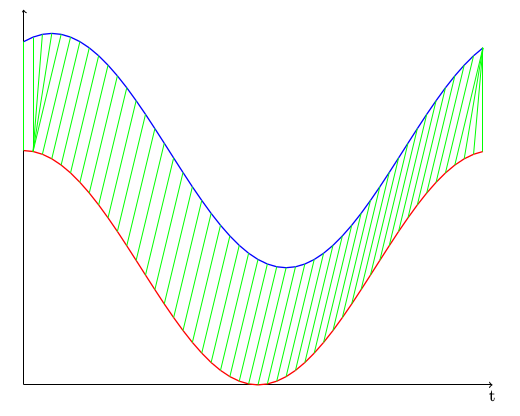
\includegraphics[scale = 0.5]{DTW2courbes.png}
\caption{Deux s\'equences en dimension $1$ align\'ees avec Dynamic Time Warping. Les coordonn\'ees de la s\'equence du haut et de celle du bas correspondent respectivement \`a
$cos(t)$ et \`a $cos(t+\alpha)$. 
Pour des questions de visualisation, la s\'equence du dessus a \'et\'e d\'ecal\'ee vers le haut lors du trac\'e. \cite{petitjean2011descriptionDTWexemple}
}
\label{DTW2courbes}
\end{figure}
% ---- figure DTW.

{\em Dynamic time warping (DTW) } est une technique pour trouver l'aligmenent optimal entre deux s\'equences d\'ependant du temps sous certaines contraintes (figure \ref{DTW2courbes}). 
Les s\'eries temporelles sont d\'eform\'ees par une transformation non-lin\'eaire de la variable temporelle, pour d\'eterminer une mesure de leur similarit\'e, ind\'ependamment de certaines transformations non-lin\'eaires du temps.
\newline
Supposons que nous souhaitons mesurer la similarit\'e entre deux s\'eries $A = (a_1, \cdots, a_m)$ et $B = (b_1, \cdots, b_m)$.
Soit $M(A,B)$ la matrice de distances entre $A$ et $B$ o\`u $M_{i,j} = (a_i - b_j)^2$.
Un chemin d'alignement {\em Dynamic Time Warping (DTW)} est une m\'ethode inspir\'ee de la distance de {\em Levenshtein}, \'egalement appel\'e {\em distance d'\'edition}. \`A l'origine, {\em DTW} \'etait appliqu\'e  dans le domaine de la reconnaissance vocale et permet de trouver l'alignement global optimal entre deux s\'equences, c'est-\`a-dire faire correspondre chaque \'el\'ement de chaque s\'equence \`a au moins un \'el\'ement de l'autre s\'equence en minimisant les co\^uts d'association. 
Le co\^ut d'une association correspond \`a la distance entre les deux \'el\'ements; classiquement une $l_p$ norm \cite{chen2004marriageLpNorm}.
La figure \ref{DTW2courbes} repr\'esente un exemple d'alignement op\'er\'e par {\em DTW}.
Il illuste l'alignement de deux sinusoides l\'eg\`erement d\'ephas\'ees. Le r\'esultat num\'erique fournit par {\em DTW} correspond \`a la somme des hauteurs des ``barreaux'' form\'es par les associations. Les extr\'emit\'es des alignements de la figure \ref{DTW2courbes} montrent que {\em DTW} est capable de r\'ealigner correctement une s\'equence par rapport \`a une autre, et parvient ainsi \`a saisir des similarit\'es que la
distance euclidienne ne peut extraire.
\newline
La distance {\em Dynamic Time Warping} est d\'efinie r\'ecursivement par :
$$
D(A_i, B_j) = \delta(A_i,B_j) + min
				\begin{cases}
				D( A_{i-1}, B_{j-1}), \\
				D( A_{i}, B_{j-1}), \\
				D( A_{i-1}, B_{j}))
				\end{cases}
$$
o\`u $A_i$ repr\'esente la sous-s\'equence $(a_1, \cdots, a_i)$. 
Le co\^ut de l'alignement optimal est alors donn\'e par
$ D(A_{|A|}, B_{|B|})$.
Le principe de programmation dynamique peut alors se r\'esoudre par un arbre en partant des
feuilles en supposant que le probl\`eme principal peut \^etre symbolis\'e par la racine et les sous-probl\`emes par des noeuds appartenant aux diff\'erents sous-arbres.
La fonction DTW peut alors \^etre m\'emois\'ee : les diff\'erents appels peuvent \^etre retenus afin de ne pas calculer deux fois la fonction appel\'ee avec les m\^emes param\`etres. 
Aussi est-il habituel, comme l'arbre contient
$| A | . | B |$ noeuds diff\'erents, de stocker ces diff\'erents r\'esultats interm\'ediaires dans une matrice $|A| \times | B |$.
Le calcul de $DTW$ consiste alors \`a trouver le chemin de co\^ut minimum dans la matrice, ce qui s'ex\'ecute avec une complexit\'e en temps et en m\'emoire de $\Theta(|A| \times |B|)$.
